\documentclass{beamer}
\usetheme{Antibes}
\usecolortheme{orchid}
%themes to test
%Theme to: AnnArbor Antibes Bergen Berkeley Berlin Boadilla boxes CambridgeUS Copenhagen Darmstadt default Dresden Frankfurt Goettingen Hannover Ilmenau Juaneged Warsaw
%Color to: albatross beaver beetle crane default dolphin dove fly lily orchiLesPins Luebeck Madrid Malmoe Marburg Montpellier PaloAlto Pittsburgh Rochester Singapore Szd rose seagull seahorse sidebartab structure whale wolverine
%Font to: default professionalfonts serif structurebold structureitalicserif structuresmallcapsserif

\usepackage{graphicx} %allows picture file insertion into document
\usepackage{ulem} %allows strikethough (\sout)
\usepackage{amsmath}
\usepackage{comment}
\usepackage{multicol}

%sets numbered citation and uses bib.bib as bibliography file
\usepackage[natbib=true, style=numeric-comp, sorting=none]{biblatex}

\renewcommand*{\bibfont}{\tiny}
\addbibresource{../references/bib.bib}
\newcommand{\pro}{\textcolor{blue}}
\newcommand{\con}{\textcolor{red}}

%NEW COMMANDS section
\newcommand{\me}{Eric W. Robbins, MD}
\newcommand{\reduce}{\href{https://doi.org/10.1001/jama.2013.5023}{REDUCE trial}}
\newcommand{\nonInf}{\href{https://doi.org/10.1056/NEJMra1510063}{``Challenges in the Design and Interpretation of Noninferiority Trials''}}
\newcommand{\triple}{LABA-ICS \& LAMA }

\setbeamerfont{footnote}{size=\tiny} %sets size of footnote citation to \tiny

\title{REDUCE Trial}
\subtitle{Limiting Steroids in COPD Exacerbations}
\author{\me}
\date{Last updated: \today}
\begin{document}
	\begin{frame}
		\maketitle
	\end{frame}
	\begin{frame}
		\frametitle{Table of Contents}
			%\begin{multicols}{2}
				\tableofcontents[hideallsubsections]
			%\end{multicols}
	\end{frame}
\section{Background}
	\subsection{History of Steroids in COPD}
		\begin{frame}{Background Studies}
			\begin{itemize}
				\item How is AECOPD Diagnosed?
				\pause
					\begin{itemize}
						\item \pro{Winnipeg criteria}:  ``cardinal'' symptoms of AECOPD
						\item Source: \href{https://doi.org/10.7326/0003-4819-106-2-196}{Winnipeg trial of antibiotics in COPD} \cite{anthonisen_antibiotic_1987}
					\end{itemize}
				\pause
				\item Where did the idea of systemic steroids come from?
				\pause
				\begin{itemize}
					\item First studies in 1950s as asthma-crosscover. Thereafter, ED studies, non-RCT trials, etc. \cite{franklin_bronchodilators_1958,beerel_controlled_1963,evans_controlled_1974,albert_controlled_1980,mendella_steroid_1982,blair_treatment_1984}
					\item First RCT to prove efficacy of systemic steroids in AECOPD was \href{https://doi.org/10.1016/S0197-2456(98)00011-7}{SCCOPE trial} \cite{erbland_systemic_1998}
					\item looked at placebo, 2 weeks, or \con{8 weeks} of steroids
				\end{itemize}
			\end{itemize}
		\end{frame}
\section{PICO Question}
	\subsection{Overview}
		\begin{frame}{PICO Question}
			\centering
			\pro{\reduce}
			\begin{tabular}{l | l}
				\hline
				\textbf{P} & Current or ex-smokers with COPD, now in exacerbation \\
				\hline
				\textbf{I} & prednisone course 5 days \\
				\hline
				\textbf{C} & prednisone course 14 days \\
				\hline
				\textbf{O} & ``clinical worsening'' \\
				\hline
			\end{tabular}
		\end{frame}
	\subsection{Population}
		\subsubsection{Inclusion Criteria}
		\begin{frame}{P: Inclusion Criteria}
			HINT: See page 2224. \\
			\pause
			\textbf{All of these:}
					\begin{itemize}
					\item Exacerbation of COPD, defined as $\geq 2$ of Winnipeg criteria:
					\begin{enumerate}
						\item $\Delta$ baseline dyspnea
						\item $\Delta$ baseline cough
						\item $\Delta$ sputum quantity or purulence
					\end{enumerate}
					\item Age $>40$ years
					\item Smoking history of $\geq 20$ pack-years
				\end{itemize}
		\end{frame}
		\subsubsection{Exclusion Criteria}
			\begin{frame}{P: Exclusion Criteria}
				HINT: See page 2224. \\
				\pause
				\textbf{Any of these:}
				\begin{itemize}
					\item History of asthma
					\item $\frac{FEV_1}{FVC} >70\%$ by bedside post-bronchodilator spirometry 
					\item Radiologic evidence of pneumonia
					\item Expected survival $<6$ months
					\item Pregnancy or lactation
					\item Inability to give written consent
				\end{itemize}
			\end{frame}
	\subsection{Intervention}
		\subsubsection{Primary Intervention}
			\begin{frame}{I: Primary Intervention}
				Further details: See page 2224, last paragraph.\\
				\begin{itemize}
					\item Randomized to a group:
					\begin{enumerate}
						\item 5-day treatment - 5-days of glucocorticoids followed by 9 days of placebo
						\item 14-day treatment - 14-days of glucocorticoids
					\end{enumerate}
					\item Glucocorticoid therapy was methylprednisolone 40 mg IV on the first
					day followed by prednisone 40 mg PO daily for the remaining days
				\end{itemize}
			\end{frame}
		\subsubsection{Secondary Intervention}
			\begin{frame}{I: Additional Treatments}
				See page 2225, subheading \textbf{``Procedures''}
				\pause
				\begin{itemize}
					\item \pro{\textbf{Additional treatments}}
					\begin{itemize}
						\item Four to six times daily \textit{PRN}, nebulized SABA
						\item Once daily inhaled LAMA (tiotropium) \textit{and} ICS/LABA (no preference)
						\item Supplemental systemic glucocorticoids could be administered at the as seen fit by treating physician
						\item 7 days of antibiotics
					\end{itemize}
				\end{itemize}				
			\end{frame}
	\subsection{Outcome}
		\begin{frame}{Outcomes}
			See page 2225.
			\pause
			\begin{block}{Primary Outcome}
				``Time to next COPD exacerbation during a follow-up of 6 months, defined as an acute clinical deterioration beyond usual day-to-day variation, \textit{requiring interaction with a clinician}.''
			\end{block}
			\begin{alertblock}{Secondary Outcomes}
				``All-cause mortality, $\Delta FEV_1$, cumulative glucocorticoid dose, and clinical performance.''
			\end{alertblock}
		\end{frame}
		\subsection{Non-Inferiority Trial}
\section{Methodology}
	\subsection{Non-Inferiority Trial}
	\subsection{Evaluating Randomization}
		\begin{frame}{Evaluating Randomization}
			Randomizaiton: See \textbf{Figure 1} (page 2224)
			\\
			Demographics: See \textbf{Table 1} (page 2226).
		\end{frame}
\section{Results}
	\subsection{Primary Outcome}
		\begin{frame}{Primary Outcome}
			See \textbf{Table 2} (page 2227) and \textbf{Figure 2} (page 2228).
			\begin{figure}
				\centering
				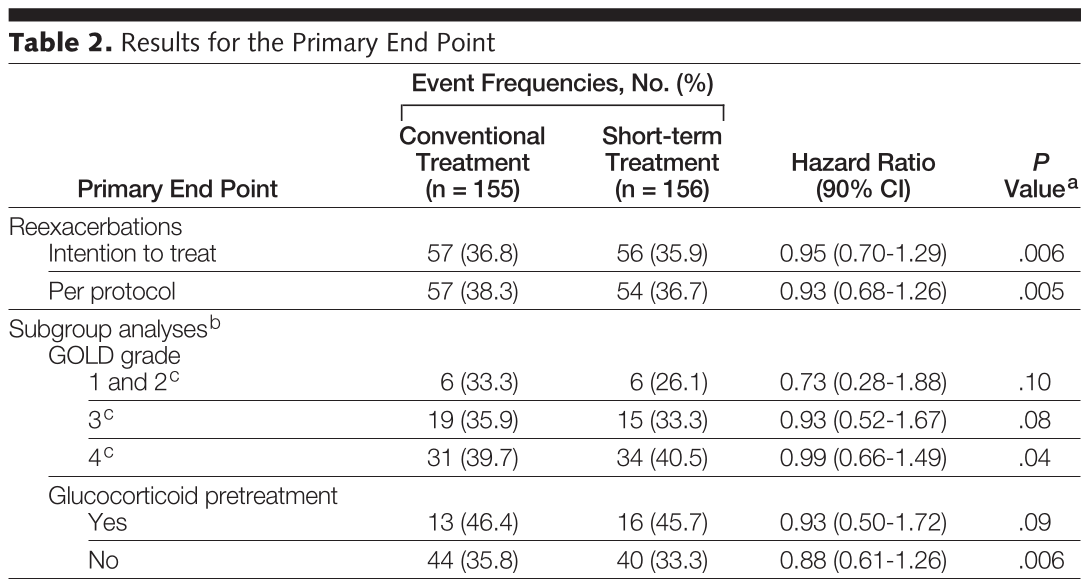
\includegraphics[width=1.0\linewidth]{../reports/figures/table2}
				\label{fig:table2}
			\end{figure}
		\end{frame}
		\begin{frame}{Primary Outcome}
			\begin{figure}
				\centering
				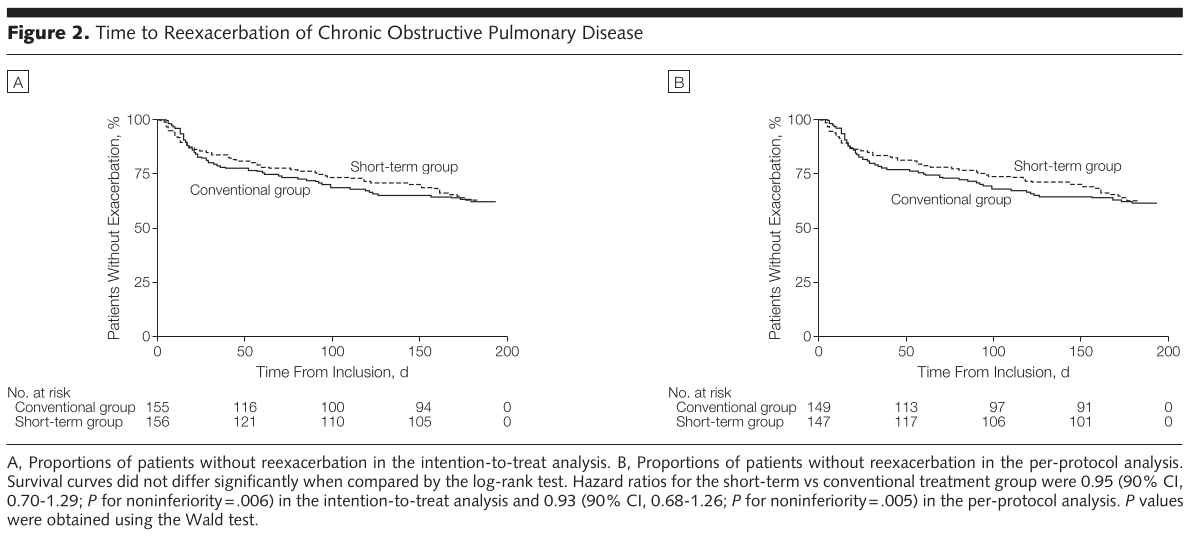
\includegraphics[width=1.0\textwidth]{../reports/figures/figure2}
				\label{fig:figure2}
			\end{figure}
		\end{frame}
	\subsection{Secondary Outcomes}
		\begin{frame}{Secondary Outcomes}
			See \textbf{Table 3} (page 2227) and \textbf{Figures 3 \& 4} (p. 2228--2229).
			\pause
			\begin{figure}
				\centering
				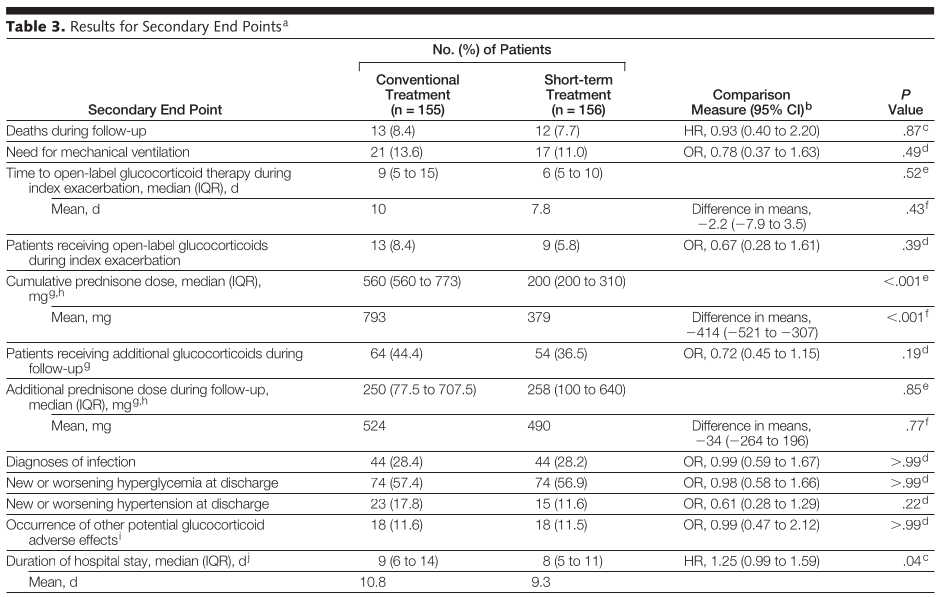
\includegraphics[width=0.90\linewidth]{../reports/figures/table3}
				\label{fig:table3}
			\end{figure}
		\end{frame}
	\subsection{Non-Inferiority}
		\begin{frame}{Our Guide}
			See second article: \\
			\nonInf. \cite{drazen_challenges_2017}
		\end{frame}
		\begin{frame}{Making Sense of Non-Inferiority}
			\begin{definition}
				``The null hypothesis in a noninferiority study states that the primary end point for the experimental treatment is worse than that for the positive control treatment \textit{by a prespecified margin}, and rejection of the null hypothesis at a prespecified level of statistical significance is used to support a claim that permits a conclusion of noninferiority.''
			\end{definition}
		\end{frame}
		\begin{frame}{Making Sense of Non-Inferiority}
			\begin{alertblock}{Requirements}
				``An acceptable noninferiority margin is defined during the design phase, which preserves a \textit{minimum clinically acceptable proportion of the effect of the active treatment} as compared with placebo. This margin cannot be greater than the smallest effect size for the active treatment that would be expected in a placebo-controlled trial.''
			\end{alertblock}
		\end{frame}
		\begin{frame}{Possible Outcomes}
			\begin{figure}
				Let's visualize!
				\centering
				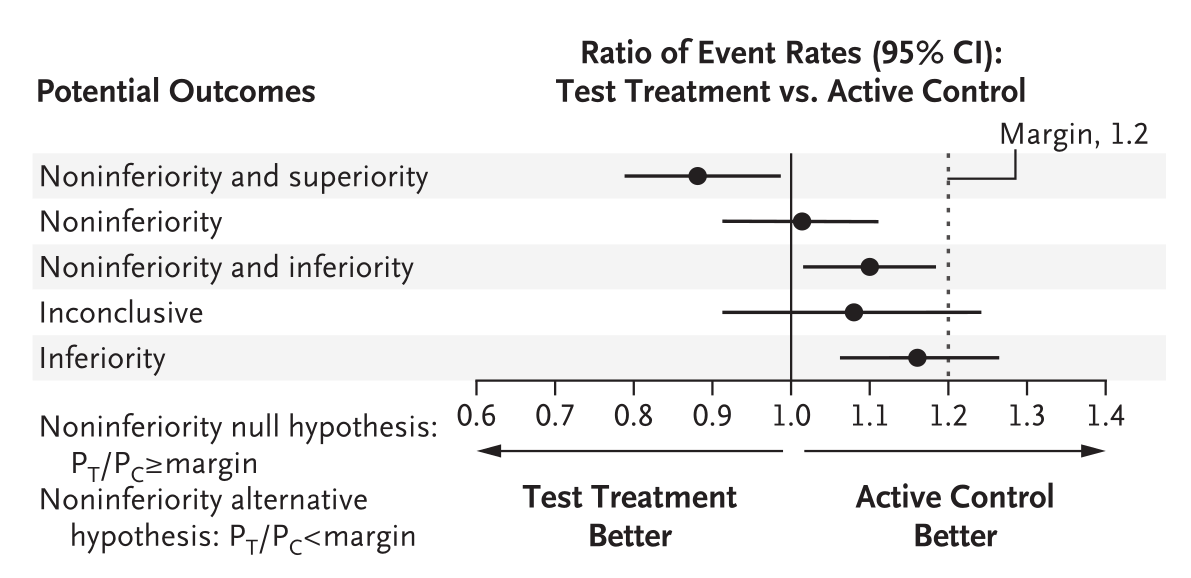
\includegraphics[width=1.0\textwidth]{../reports/figures/noninferiority-outcomes}
				\label{fig:noninferiority-outcomes}
			\end{figure}
		\end{frame}
	\subsection{Hazards of Interpreting Non-Inferiority}
		\begin{frame}{Hazards of Interpreting Non-Inferiority}
			See second article, Tables 1 and 2: \\
			\nonInf.
		\end{frame}
	\subsection{Our Study}
		\begin{frame}{Our Study: Deciding Non-Inferiority}
			\begin{alertblock}{\reduce, Non-Inferiority Definition}
				``\con{Based on the judgement of 11 board-certified specialists}, we defined a 15\% absolute difference in the percentage of patients with a reexacerbation during the 6 months of follow-up as the clinically tolerable upper limit. Based on previously published data,we assumed that approximately 50\% of patients would experience an exacerbation during follow-up.
				\\
				Therefore...the true proportion of patients...experiencing a COPD exacerbation must not exceed 65\%...which translates to a \pro{critical hazard ratio (HR) of 1.515}...''
			\end{alertblock}
		\end{frame}
		\begin{frame}{Deciding Non-Inferiority, Continued}
			\begin{alertblock}{\reduce,  Non-Inferiority Definition}
				Noninferiority was concluded if the 2-sided, \textbf{90\% confidence interval} for the HR between the short-term and the conventional treatment group in an intention-to-treat and per-protocol analysis was below 1.515, which corresponds to an $\alpha$ level of 5\%.
			\end{alertblock}
		\end{frame}
\section{Criticisms}
	\begin{frame}{Criticisms}
		Thoughts?
		\pause
		\begin{itemize}
			\item \textbf{Randomization}
			\begin{itemize}
				\item significant between-group difference in sex representation
			\end{itemize}
			\item \textbf{External validity}
			\begin{itemize}
				\item Do we always give \triple inhalers?
				\item Broad-spectrum antibiotics with NO radiographic pneumonia?
			\end{itemize}
			\item \textbf{Results Interpretation}
			\begin{itemize}
				\item Primary outcome shown as Kaplan-Meier, not Forest plot
				\item 90\% confidence interval is not usual
			\end{itemize}
		\end{itemize}
	\end{frame}
\section{Discussion}
	\begin{frame}{Discussion}
		\begin{itemize}
			\item Does this change your \textit{default} steroid course length?
			\item Would you now be more likely to:
				\begin{itemize}
					\item Consider course of steroids $\geq 5$ days?
					\item Continue (or start?) \triple inhalers?
					\item Give broad-spectrum antibiotics?
				\end{itemize} 
		\end{itemize}
	\end{frame}
\section*{References}
	\begin{frame}[allowframebreaks]{References}
		\printbibliography
	\end{frame}
\end{document}